\subsection{Mean Shift}
\label{sec:Mean Shift}
\textit{written by Leonie Bender}
\\

Mean Shift is an algorithm which can be used to find distinct clusters within a given data set. 
The method was first proposed in 1975 by Fukunaga and Hostetler \cite{fukunaga1975estimation} and is categorized as density-based clustering.
It is assumed that data points of a given data set are sampled from a distribution, the probability density function. The main idea is to define clusters in dense regions of the feature space. Therefore, clusters are defined around centroids corresponding to peaks, so-called \textit{modes}, of the underlying probability density function. Mean Shift makes use of the concept of kernel density estimation, as the underlying distribution, which determines the cluster centroids, is not given. Local structures of the estimated probability density function influence both, the number of resulting clusters as well as which data points are assigned to which cluster \cite{comaniciu2002MeanShift}.  \\
The only input the user has to provide for Mean Shift Clustering is the \textit{bandwidth} or \textit{scale} \cite{scikit-learn}. The bandwidth parameter \textit{h $>$ 0} determines the kernel's radius. During density estimation procedure, the kernel is located at each point in feature space and data density at the respective point is estimated taking into account the number of data points included inside the kernel's bandwidth. Thus, the larger the bandwidth is chosen, the larger is the kernel's radius, resulting in a smoother estimated density surface. Analogously, the smaller the bandwidth is chosen, the smaller is the kernel's radius and hence this results in an estimated density surface containing a peak for almost each point (Figure \ref{fig:kde_estimation}).
Accordingly, if the bandwidth parameter value is chosen too small, Mean Shift will assign each data point to it's own cluster. In contrast to that, if the bandwidth parameter is chosen too large, Mean Shift will assign all data points to one single cluster. 
\begin{figure}[H]
\centering
    \subfigure{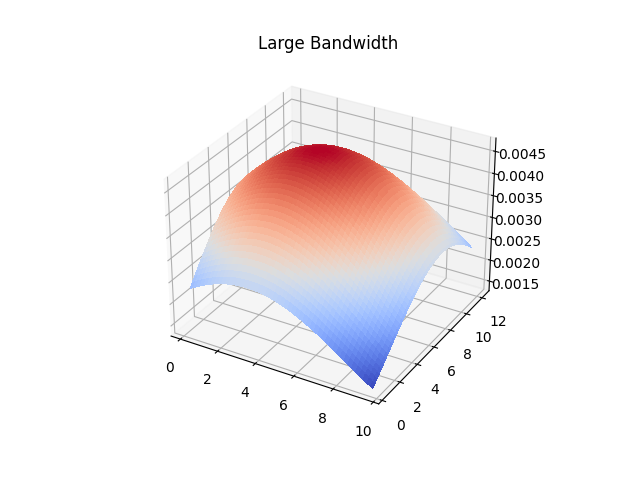
\includegraphics[width=0.3\linewidth]{images/Surface_5.png}}
    \subfigure{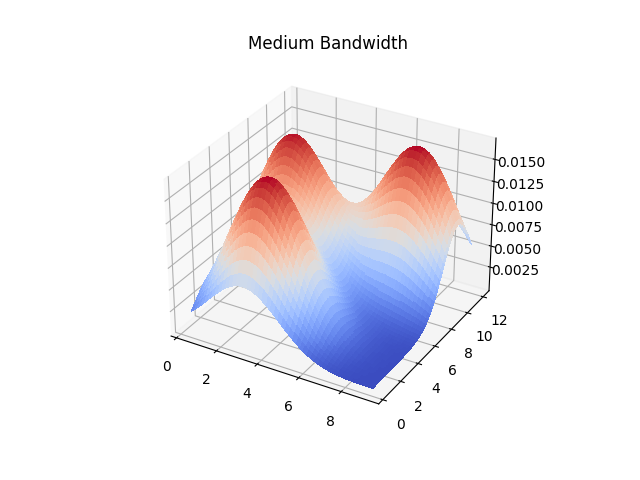
\includegraphics[width=0.3\linewidth]{images/Surface_1_5.png}}
    \subfigure{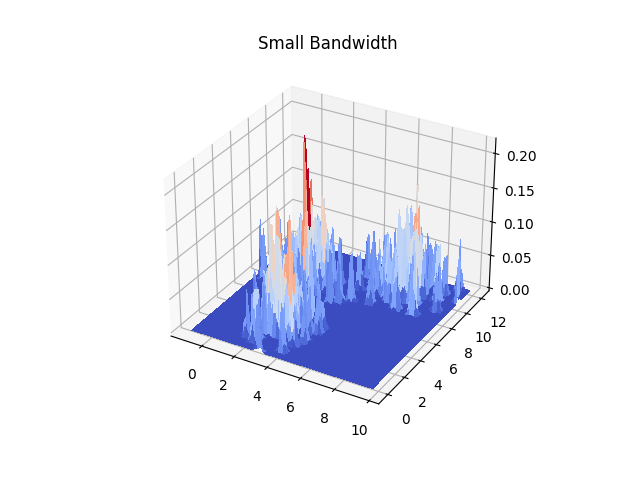
\includegraphics[width=0.3\linewidth]{images/Surface_0_1.png}}
    \caption{Influence of Bandwidth Parameter on Estimated Density Surface}
    \label{fig:kde_estimation}
\end{figure}

For a given data set consisting of \textit{n} data points in the \textit{d}-dimensional space, the kernel density estimator, using kernel $K(x)=c_{k, d} \cdot k \left( ||x||^{2} \right)$ with bandwidth \textit{h $>$ 0}, is given through\\
\begin{align*}
	\hat{f}_{h, K} = \frac{c_{k, d}}{n \cdot h^{d}} \sum_{i=1}^{n} k \left( \left|\left|\frac{x - x_{i}}{h} \right|\right|^{2}\right).
\end{align*}
As explained above, modes of this density have to be found as each mode determines one cluster centroid. Modes correspond to stationary points which fulfill the requirement that $\nabla \hat{f}(x) \overset{!}{=} 0$. Computing the gradient of the estimated density function $\hat{f}$ and afterwards performing some further algebraic manipulations yields the following formula:
\begin{align*}
	\hat{\nabla} f_{h,K}(x) = \underbrace{\frac{2 \cdot c_{k, d}}{n \cdot h^{d+2}} \left[ \sum_{i=1}^{n} g \left( \left| \left| \frac{x-x_{i}}{h} \right| \right| ^{2} \right) \right]}_{\text{proportional to $\hat{f}_{h, K}$}}\underbrace{ \left[ \frac{\sum_{i=1}^{n} x_{i} \cdot g \left( \left| \left| \frac{x-x_{i}}{h} \right| \right| ^{2} \right)}{\sum_{i=1}^{n} g \left( \left| \left| \frac{x-x_{i}}{h} \right| \right| ^{2} \right)} - x \right]}_{\text{mean shift}}.
\end{align*}
While the first term is proportional to the above stated density estimate at point x, the second term describes the actual mean shift. It denotes the shift of point x, on which the kernel center is located, to the weighted mean of all the neighboring data points inside the kernel's bandwidth. It can be shown that the mean shift vector always points in the direction of maximal increase of density of data points \cite{comaniciu2002MeanShift}. 
Local peaks of the probability density function are thus found by iteratively performing the mean shift as a gradient ascent method.\\
The iterative mean shift approach therefore provides a way to determine modes without having to estimate the complete density function beforehand \cite{comaniciu2002MeanShift}.

Initially, each of the given data points is chosen to be a candidate cluster centroid. In each iteration, all the candidate centroids are updated by shifting them to the mean of their respective neighboring data points. As the mean shift vector always points into the direction of maximal increase, repeating this procedure finally locates local maxima of the density function.
The lower the density of data points, the larger the mean shift steps get. Thus, data point density automatically regulates the step size and therefore, mean shift is an adaptive form of a gradient ascent method. 
After the mean shift of each data point is performed, the next iteration starts by placing the kernel's center on the shifted data point and again shifting it to the mean of its respective neighbors \cite{400568}. 

The algorithm stops if the shift of centroids falls below a predefined threshold. All data points that reside at the same stationary point are summarized into the same cluster where the local maximum of the underlying density function is used as the cluster centroid. 
One can imagine that each data point is shifted to its nearest local peak of the density function and all data points located at the same maximum are assigned to the same cluster around this mode.

The procedure of Mean Shift Clustering can be summarized by the following pseudocode:
\begin{algorithm}[H]
	\caption{Mean Shift Clustering} 
	\begin{algorithmic}[1]
		\For {$i$=1, \ldots, N}
			\While{$mean$ $shift$ $exceeds$ $threshold$}
				\State $m(x_{i})\leftarrow compute$ $mean$ $of$ $neighboring$ $data$ $points$ $of$ $x_{i}$
				\State $x_{i}\leftarrow m(x_{i})$
			\EndWhile
			\State Store $z_{i}\leftarrow x_{i}$ 
		\EndFor
		\State Identify clusters $\{C\}_{1\ldots m}$ grouping together all nearby $z_{i}s$ 
		\State Return clusters $\{C\}_{1 \ldots m}$
	\end{algorithmic} 
\end{algorithm}

As the search for all the neighboring data points is computationally costly and in each iteration a large number of such searches has to be performed, the algorithm is not highly scalable. While in lower dimensions, complexity tends towards $O(T \cdot n \cdot log(n))$, in higher dimensions complexity tends towards $O(T \cdot n^{2})$, where \textit{n} denotes the number of samples and \textit{T} denotes the number of data points. If all given data points are used as samples, this results in a complexity of $O(n^{2} \cdot log(n))$ in lower dimensions and analogously to a complexity of $O(n^{3})$ in high dimensions. This complexity can be improved by initializing only a fraction of data points as candidate cluster centroids or by only taking a subset of all the given data points as samples \cite{sklearn_api}. Details on this are provided in section \ref{subsec:sklearn_meanshift}. \\
Unlike other clustering algorithms, Mean Shift is a nonparametric method, meaning it neither makes any assumption on the number of resulting clusters nor on their shape. Thus, the algorithm can be used to find clusters of arbitrary, even non-elliptical shapes. This makes Mean Shift applicable to real world data sets where clusters of convex shapes would possibly introduce severe artifacts \cite{comaniciu2002MeanShift}.\\
In addition to that, Mean Shift Clustering is robust against outliers. This can be verified as outliers would only lead to the definition of a cluster consisting of a single data point instead of shifting the centroid of another cluster.
At the same time, this can also be seen as a disadvantage of the Mean Shift algorithm. The resulting clusters caused by outliers are not meaningful and do not have any reasonable interpretation when analyzing the resulting clustering. 
The rationale of another drawback of Mean Shift algorithm is based on the concept of kernel density estimation. In high dimensions, kernel density estimation may react sensitively to changes of the bandwidth parameter value. Therefore, Mean Shift Clustering is better applicable to low-dimensional data sets as well as data sets consisting of dense regions \cite{CarreiraPerpin2015ARO}.